\section{ขั้นตอนวิธีเชิงตัวเลขที่นำเสนอ}
\subsection{ขั้นตอนวิธีเชิงตัวเลขสำหรับต่อเติมภาพศิลปะ}

\hspace{1cm} สำหรับวิธีการซ่อมแซมภาพสิลปะไทย จะใช้วิธีการสปริทเบรกแมนเพื่อหลีกเลี่ยงปัญหาเชิงตัวเลขที่จะเกิดขึ้น แต่เพื่อให้วิธีการสปริทเบรกแมนประมวลผลภาพได้รวดเร็วขึ้น ผู้วิจัยได้พัฒนากระบวนการกำหนดคำตอบเริ่มต้นโดยวิธีการมัลติรีโซลูชัน (multi-resolution method) หรือวิธีการพีระมิดรูปภาพ (pyramid method) \cite{ref:image-pyramid}
เริ่มจากการย่อขนาดรูปลงครึ่งนึงโดยใช้วิธี Bilinear Interpolation จนกระทั่งถึงระดับ \break ความคมชัดที่ต้องการ จากนั้นทำการต่อเติมภาพขนาดเล็ก และนำผลลัพธ์ที่ได้จากภาพขนาดเล็กทำการขยายภาพขึ้นสองเท่าโดยใช้ Bilinear Interpolation เป็นคำตอบเริ่มต้นสำหรับการต่อเติมภาพในชั้นถัดไป
\begin{figure}[H]
    \centering
    \begin{subfigure}{0.4\linewidth}
        \centering
        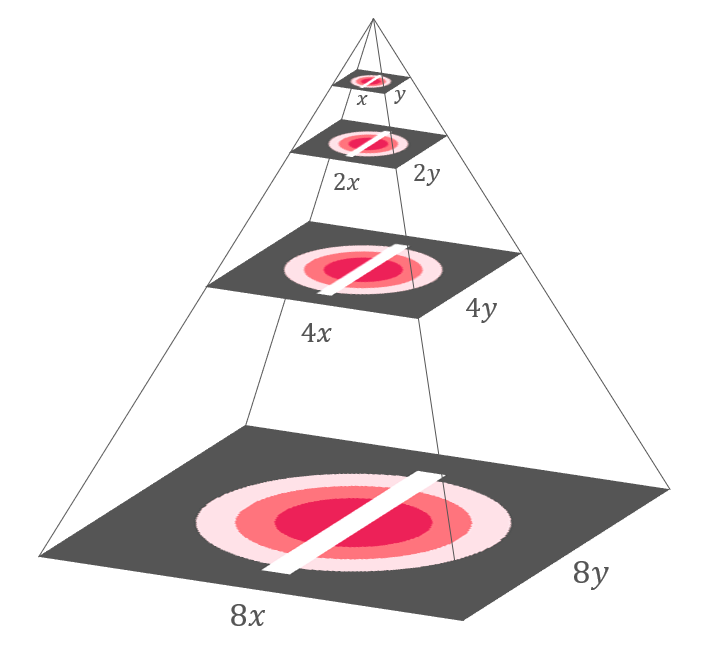
\includegraphics[width=0.8\linewidth]{image/image_inpaint_synthetic/image_pyramid.png}
    \end{subfigure}
     \caption{วิธีการพีระมิดรูปภาพ}
\end{figure}
\hspace{1cm} ขั้นตอนวิธีสำหรับการทำพีระมิดรูปภาพสำหรับการต่อเติมภาพแบบสปริทเบรกแมนเพื่อให้ประมวลผลได้เร็วขึ้นนั้นสามารถสรุปได้ดังนี้\\


\begin{algorithm}[H]
    \label{algorithm:MultiSplitBregmanColorInpaint}
    \caption{วิธีสปริทเบรกแมนที่ใช้พีระมิดรูปภาพ}
    \KwIn{
        \\
        \hspace{1cm} $u$ คือรูปภาพที่ต้องการต่อเติม \\
		\hspace{1cm} $\lambda$ คือพารามิเตอร์เร็กกิวลาร์ไรเซชัน ที่ได้กล่างถึงในสมการ (\ref{e2}) \\
        \hspace{1cm} $\theta$ คือพารามิเตอร์เพนัลที ซึ่งเป็นจำนวนจริงบวก\\
        \hspace{1cm} $N_{gs}$ เป็นจำนวนเต็มบวกสำหรับกำหนดจำนวนรอบที่ทำงานของการทำเกาส์-ไซเดล \\
        \hspace{1cm} $c$ ตัวแปรช่วยสำหรับบอกความลึก ให้กำหนดเป็น 1 \\
        \hspace{1cm} $m$ คือ ระดับความลึกของพีระมิดรูปภาพ เป็นจำนวนเต็มบวก \\
        \hspace{1cm} $N_0$ จำนวนรอบการทำสปริทเบรกแมนที่ชั้นละเอียดสุด \\
        \hspace{1cm} $N_1$ จำนวนรอบการทำสปริทเบรกแมนที่ชั้นต่างๆ \\
        \hspace{1cm} $N_2$ ตำนวนรอบการทำสปริทเบรกแมนที่ชั้นหยาบสุด \\
	}
	\KwOut{รูปภาพที่ผ่านการต่อเติมแล้ว}
    \SetAlgoNoLine
    \SetKwFunction{FMain}{$u \longleftarrow MultiSplitBregmanColor $}
    \SetKwProg{Fn}{}{}{}
    \Fn{\FMain{$\boldsymbol{u}, \lambda, \theta, N_{gs}, N_0,N_1,N_2, \varepsilon,c,m$}}{
        \textbf{Initialize} $height = $ ความสูงของภาพ $\boldsymbol{u}$, $width = $ ความกว้างของภาพ $\boldsymbol{u}$ \\
        \If{c < m}{
            $\boldsymbol{x} = Bilinear(\boldsymbol{u},\lfloor width * 0.5 \rfloor,\lfloor height * 0.5 \rfloor)$\\
            $y = Bilinear(\lambda,\lfloor width * 0.5 \rfloor,\lfloor height * 0.5 \rfloor)$\\
            $r = MRSBC(\boldsymbol{x},\boldsymbol{z},y, \lambda, \theta,$ \\$ \hspace{1cm}  N_{gs}, N_0, N_1, N_2, \varepsilon,c+1,m)$\\
            $\boldsymbol{u} = Bilinear(r,width,height)$\\
        }
        \uIf{$c = 1$}{$N_{SB}=N_0$}
        \uElseIf{$c = m$}{$N_{SB} = N_2$}
        \Else{
            $N_{SB} = N_1$
        }
        $u = SplitBregmanColor(\boldsymbol{u}, \lambda, \theta, N_{gs}, N_{SB}, \varepsilon) $  \\
    }
\end{algorithm}

\vspace{0.5cm}

\begin{algorithm}[H]
    \caption{Bilinear Interpolation}
    \SetAlgoNoLine
    % https://stackoverflow.com/questions/26142288
    \SetKwFunction{FMain}{$J \longleftarrow Bilinear$}
    \SetKwProg{Fn}{}{}{}
    \Fn{\FMain{$I,x,y$}}{
        \textbf{Initialize}  $v =$ ความสูงของภาพ $I$, $w$ คือความกว้างของภาพ $I$,\\ $S_R = \frac{c}{a}, S_C = \frac{d}{b}, r = 1,2,...,v, c = 1,2,...,w,$\\$r' = 1,2,...x, c' = 1,2,...,y,  $ \\
        $r_f = \lfloor r' \cdot S_R \rfloor $\\
        $c_f = \lfloor c' \cdot S_C \rfloor $\\
        $\triangle r = r_f - r$ \\
        $\triangle c = c_f - c$ \\
        $J(r',c') = I(r,c)\cdot(1-\triangle r)\cdot (1-\triangle c) $\\$+ I(r+1,c) \cdot \triangle r \cdot (1 - \triangle c) $\\$+I(r,c+1)\cdot(1-\triangle r)\cdot\triangle c$\\$+ I(r+1,c+1)\cdot\triangle r \cdot \triangle c$ \\
    }
\end{algorithm}

\hspace{1cm} นอกจากนี้แล้ว ผู้วิจัยได้สังเกตว่า การทำซ้ำจะลู่เข้าเร็วในช่วงแรก จากนั้นความเร็วในการลู่เข้าจะลดลง ซึ่งทำให้เราสามารถใช้จำนวนรอบของการทำซ้ำเพียงไม่กี่ครั้งในระดับความคมชัดเดิมเพื่อซ่อมแซมภาพ



\begin{figure}[H]
    \centering
    \begin{subfigure}{0.4\linewidth}
        \centering
        
\includegraphics[width=0.53\linewidth]{image/just10enough/only5time.png}
        \caption{5 ครั้ง}
    \end{subfigure}
    \begin{subfigure}{0.4\linewidth}
        \centering
        
\includegraphics[width=0.53\linewidth]{image/just10enough/only10time.png}
        \caption{10 ครั้ง}
    \end{subfigure}
    \begin{subfigure}{0.4\linewidth}
        \centering
        
\includegraphics[width=0.53\linewidth]{image/just10enough/only50time.png}			
        \caption{50 ครั้ง}
    \end{subfigure}
    \begin{subfigure}{0.4\linewidth}
        \centering
        
\includegraphics[width=0.53\linewidth]{image/just10enough/only100time.png}			
        \caption{100 ครั้ง}
    \end{subfigure}
    \caption{ผลการซ่อมแซมภาพวิเคราะห์เมื่อใช้จำนวนรอบในการทำซ้ำที่ระดับความคมชัดสูงสุดซึ่งมีค่าต่างกัน}
    \label{figure:just-ten-enough}

\end{figure}

\hspace{1cm} 
จากรูปที่ \ref{figure:just-ten-enough}
แสดงให้เห็นถึงจำนวนรอบการทำซ้ำที่ความคมชัดสูงสุด 10 ครั้งเพียงพอต่อการซ่อมแซมภาพจนมีผลการซ่อมแซมภาพที่ดี นอกจากนี้เรายังพบจากการตรวจสอบว่าการใช้จำนวนรอบของการทำซ้ำในระดับความคมชัดต่ำยังทำให้ผลการทำงานในภาพรวดเร็วขึ้นอย่างมีนัยยะสำคัญ

\subsection{ขั้นตอนวิธีเชิงตัวเลขสำหรับซ่อมแซมภาพวิดีโอ}

\hspace{1cm}เนื่องจากไฟล์วิดีโอนั้นประกอบด้วยชุดของภาพหลายภาพ กล่าวคือ $V = \{\boldsymbol{u}_i| i = 1,2,3 ... N_f\}$ ทำให้ขั้นตอนการลบบทบรรยายออกจากวิดีโอ จะต้องทำการต่อเติมภาพในบริเวณที่เป็นบทบรรยายทีละภาพ \break ดังที่แสดงในขั้นตอนวิธีต่อไปนี้ \\
	
\begin{algorithm}[H]
    \caption{Removing subtitle from video}	
    \SetAlgoNoLine
    \SetKwFunction{FMain}{$V \longleftarrow RemoveS$}
    \SetKwProg{Fn}{}{}{}
    \Fn{\FMain{$V$}}{
        \For{$ i = 1,2,... N_f$}{
            $\bullet$ หาโดเมนต่อเติม $D$ จาก $\boldsymbol{u}_i$\\
            $\bullet$ ต่อเติมภาพ $\boldsymbol{u}_i$ โดยใช้โดเมนต่อเติม $D$\\
        }
    }
\end{algorithm}

\vspace{1cm}
\hspace{1cm} ขั้นตอนการต่อเติมภาพ $\boldsymbol{u}_i$ ในโดเมนต่อเติม $D$ สามารถใช้วิธีการเดียวกับการซ่อมแซมภาพศิลปะไทยได้ ส่วนการหาโดเมนต่อเติมซึ่งเป็นบทบรรยายอนิเมะจะกล่าวถึงในหัวข้อย่อยถัดไป

\subsection{การหาบทบรรยายบนอนิเมะ}	
\hspace{1cm}ก่อนจะลบบทบรรยายนั้น จำเป็นต้องหาบทบรรยายในภาพให้ได้เสียก่อน โดยบทบรรยายของอนิเมะนั้น มักจะใช้ขอบของตัวอักษรสีดำ อีกทั้งบทบรรยายนั้นมีตำแหน่งห่างออกมาจากขอบของวิดีโอ และขนาดของบทบรรยายนั้นจะมีขนาดเล็กเมื่อเทียบกับเฟรมภาพ ด้วยสมบัตินี้เองทำให้จึงสามารถหาบริเวณบนเฟรมที่เป็นบทบรรยายได้โดยใช้ขั้นตอนวิธีที่สรุปดัง Algorithm \ref{algorithm:FindSubtitle} ดังนี้
	
\vspace{1cm}

\begin{algorithm}[H]
    \caption{Finding subtitle}
    \SetKwFunction{FMain}{$D \longleftarrow findsub$}
    \SetAlgoNoLine
    \SetKwProg{Fn}{}{}{}
    \Fn{\FMain{$\boldsymbol{u}$}}{
        $\bullet$ ทำการเปลี่ยนสีดำในภาพ $\boldsymbol{u}$ ให้เป็นสีขาวแล้วเปลี่ยนอื่นๆ ให้เป็นสีดำเพื่อหาขอบของคำบรรยาย\\
        $\bullet$ เปลี่ยนบริเวณสีขาวในภาพให้เป็นสีดำ และเปลี่ยนบริเวณสีดำให้เป็นสีขาว\\
        $\bullet$ ทำการลบบริเวณสีขาวซึ่งติดกับขอบของภาพออกไป เนื่องจากบทบรรยายจะลอยอยู่ ไม่ติดกับขอบเสมอ\\
        $\bullet$  ลบบริเวณที่ใหญ่เกินกว่าจะเป็นบทบรรยาย \\
        $\bullet$  ลบบริเวณที่เล็กเกินกว่าจะเป็นบทบรรยาย \\
        $\bullet$ ทำการขยายพื้นที่ๆ เป็นสีขาวขึ้นด้วยความกว้างของขอบบทบรรยาย \\
        $\bullet$ สีขาวที่เหลืออยู่ในภาพจะเป็นบทบรรยาย
    }	
    \label{algorithm:FindSubtitle}
\end{algorithm}

\subsection{การลบบทบรรยายจากบทอนิเมะ}

\hspace{1cm} เพื่อเร่งการลบบทบรรยาย เราสามารถใช้ผลการต่อเติมภาพจากเฟรมก่อนหน้า มาใช้เป็นคำตอบเริ่มต้นของเฟรมปัจจุบัน จึงได้ว่า\\
	
\vspace{0.5cm}
\begin{algorithm}[H]
    \SetAlgoNoLine
    \caption{วิธีการทำงานบนวิดีโอ เมื่อต้องการผลจากภาพที่แล้วมาใช้เป็นคำตอบเริ่มต้น}
    \SetKwFunction{FMain}{$V \longleftarrow RemoveSubtitle$}
    \SetKwProg{Fn}{}{}{}
    \Fn{\FMain{$V$}}{
        \textbf{initialize} $i =1$\\
        \While{$i < N_f - 1$}{
            $\boldsymbol{u}_i$ คือเฟรมที่ $i$ ใน $V$ \\
            $\boldsymbol{u}_{i+1}$ คือเฟรมที่ $i+1$ ใน $V$ \\
            $D$ คือโดเมนต่อเติมใน $\boldsymbol{u}_{i+1}$ \\
            $\boldsymbol{u}_{i+1} = RemoveByBorrowFrame(\boldsymbol{u}_{i},D,\boldsymbol{u}_{i+1})$
        }
    }	
\end{algorithm}
\vspace{0.5cm}



\vspace{0.5cm}	
\hspace{1cm} นอกจากนี้เราสามารถใช้แนวคิดของการยืมข้อมูลจากเฟรมที่เกี่ยวข้องเพื่อเป็นข้อมูลเริ่มต้นในการเร่งการประมวลผลได้ดังนี้ \\
	
\vspace{0.5cm}
\begin{algorithm}[H]
    \SetAlgoNoLine
    \label{algorithm:subtitle_borrowframe}
    \caption{การลบบทบรรยายโดยใช้วิธีการยืมเฟรม}  
    \SetKwFunction{FMain}{$\boldsymbol{v} \longleftarrow RemoveByBorrowFrame$}
    \SetKwProg{Fn}{}{}{}
    \Fn{\FMain{$\boldsymbol{u} , D, \boldsymbol{v} $}}{
        $s =$ ค่า SSIM ระหว่าง  $\boldsymbol{u}$ และ $\boldsymbol{v}$  บริเวณนอกโดเมนต่อเติม\\
        \If{s > 0.9}{
            คัดลอกบริเวณในโดเมนต่อเติมจาก $\boldsymbol{u} $ ไปยัง $\boldsymbol{v}$
        }
        $\boldsymbol{v} = MultiSplitBregmanColor(\boldsymbol{v},\lambda, \theta, N_{gs}, N_0, N_1, N_2, \varepsilon,1,m)$
    }	
\end{algorithm}
 
\vspace{0.5cm}
\begin{algorithm}[H]
    \SetAlgoNoLine
    \label{algorithm:subtitle_skipframe}
    \caption{Removeing subtitle from video (Method 3)}  
    \SetKwFunction{FMain}{$\boldsymbol{v}, \longleftarrow removeS3$}
    \SetKwProg{Fn}{}{}{}
    \Fn{\FMain{$\boldsymbol{u}, D, \boldsymbol{v}$}}{
        $s =$ ค่า SSIM ระหว่าง  $\boldsymbol{u}$ และ $\boldsymbol{v}$  บริเวณนอกโดเมนต่อเติม\\
        \uIf{s > 0.95}{
            คัดลอกบริเวณในโดเมนต่อเติมจาก $\boldsymbol{u}$ ไปยัง $\boldsymbol{v}$
        }
        \Else{
            $\boldsymbol{v} = MRSBC(\boldsymbol{u} ,\boldsymbol{z} ,\lambda, \theta, N_{gs}, N_0, N_1, N_2, \varepsilon,1,m)$
        }
    }	
\end{algorithm}
\vspace{0.5cm}

\vspace{0.5cm}
\begin{algorithm}[H]
    \label{algorithm:subtitle_skipnborrowframe}
    \caption{Removing subtitle from video (Method 4)}  
    \SetAlgoNoLine
    \SetKwFunction{FMain}{$\boldsymbol{v} \longleftarrow removeS4$}
    \SetKwProg{Fn}{}{}{}
    \Fn{\FMain{$\boldsymbol{u} , D, \boldsymbol{v} $}}{
        $s =$ ค่า SSIM ระหว่าง  $u$ และ $v$  บริเวณนอกโดเมนต่อเติม\\
        \uIf{s > 0.95}{
            คัดลอกบริเวณในโดเมนต่อเติมจาก $\boldsymbol{u} $ ไปยัง $\boldsymbol{v}$
        }
        \uElseIf{s > 0.9}{
            คัดลอกบริเวณในโดเมนต่อเติมจาก $\boldsymbol{u} $ ไปยัง $\boldsymbol{z}$\\
            $\boldsymbol{v} = MRSBC(\boldsymbol{u} ,\boldsymbol{z} ,\lambda, \theta, N_{gs}, N_0, N_1, N_2, \varepsilon,1,m)$
        }\Else{
            $\boldsymbol{v} = MRSBC(\boldsymbol{u} ,\boldsymbol{z} ,\lambda, \theta, N_{gs}, N_0, N_1, N_2, \varepsilon,1,m)$
        }
    }	
\end{algorithm}

